
% Reference: https://tex.stackexchange.com/questions/8827/preparing-cheat-sheets/8915

% Package imports.
\documentclass[10pt,landscape]{article}
\usepackage{multicol}
\usepackage{calc}
\usepackage{ifthen}
\usepackage[landscape, a4paper]{geometry}
\usepackage{amsmath,amsthm,amsfonts,amssymb}
\usepackage{color,graphicx,overpic}
\usepackage{hyperref}
\newenvironment{Figure}
{\par\medskip\noindent\minipage{\linewidth}}
{\endminipage\par\medskip}

% Sets page margins.
\geometry{top=.2in,left=.2in,right=.2in,bottom=.2in}

% Turns off header and footer.
\pagestyle{empty}

% Redefine section commands to use less space and have smaller text.
% (Can change font size if `\tiny` is too small.
% See http://www.sascha-frank.com/latex-font-size.html as a reference.)
\makeatletter
\renewcommand{\section}{\@startsection{section}{1}{0mm}%
                                {-0.5ex plus -.5ex minus -.2ex}%
                                {-0.5\baselineskip}%
                                {\normalfont\small\bfseries}}
\renewcommand{\subsection}{\@startsection{subsection}{2}{0mm}%
                                {-0.5ex plus -.5ex minus -.2ex}%
                                {-0.5\baselineskip}%
                                {\normalfont\small\bfseries}}
\renewcommand{\subsubsection}{\@startsection{subsubsection}{3}{0mm}%
                                {-0.5ex plus -.5ex minus -.2ex}%
                                {-0.5\baselineskip}%
                                {\normalfont\small\bfseries}}
\renewcommand{\paragraph}{\@startsection{paragraph}{4}{0mm}%
                                {-0.5ex plus -.5ex minus -.2ex}%
                                {-0.5\baselineskip}%
                                {\normalfont\small\bfseries}}
\makeatother

% No section numbers.
\setcounter{secnumdepth}{0}

% Minimal paragraph indenting and spacing.
\setlength{\parindent}{0pt}
\setlength{\parskip}{0pt plus 0.5ex}

% Canonical "init" statement.
\begin{document}

% Don't start new paragraphs if you don't need to.
\raggedright

% Font size.
\scriptsize

% Specifying number of columns.
% Asterisk "*" here to force the left-most column to fill first, then the next, ect.
% (Otherwise, all columns would fill down "equally".
\begin{multicols*}{4}

% Can play around with these as desired.
\setlength{\columnseprule}{0.25pt}
\setlength{\premulticols}{0.25pt}
\setlength{\postmulticols}{0.25pt}
\setlength{\multicolsep}{0.25pt}
\setlength{\columnsep}{0.25pt}

% This is the "magic" pandoc variable. (This is where your Rmarkdown document is inserted.)
\section{2. Linear Algebra}

1. $Injective$ iff f(x1) = f(x2) implies that x1 = x2.\\
2. $Surjective$ iff for all $y \in Y$ there exists $x \in X$ such that y = f(x).\\
3. $Bijective$ iff it is both injective and surjective, i.e. for all $y \in Y$ there exists a unique $x \in X$ such that y = f(x).\\

1. f has a left inverse iff it is injective.\\
2. f has a right inverse iff it is surjective.\\
3. f is invertible iff it is bijective.\\
4. If f is invertible then any two inverses (left-, right- or both) coincide.\\

\textbf{Group} (G, *):\\
1. $Associative \forall a, b, c \in G, a * (b * c) = (a * b) * c$.\\
2. $Identity: \exists e \in G, \forall a \in G, a * e = e * a = a.$\\
3. $Inverse: \forall a \in G, \exists a^{-1} \in G, a * a ^{-1} = a^{-1} * a = e.$\\
(G, *) is commutative (or Abelian) iff in addition to 1-3:\\
4. $Commutative: \forall a, b \in G, a * b = b * a.$\\

\textbf{Ring} (R, +, $\cdot$):\\
$+: associative, identity, inverse, communtative$\\
$\cdot : associative, identity$\\
$distributive: a \cdot (b+c) = a \cdot b + a \cdot c and (b + c) \cdot a = b \cdot a + c \cdot a$\\

\textbf{Field} is a $communitative\ Ring$ that in addition satisfies $Multiplication\ inverse.$\\

\textbf{Linear Space} $(V, F, \oplus, \odot)$:
$\oplus: associative, identity, inverse, communtative (V!!)$\\
$\odot: associative \forall a,b \in F, x \in V, a \odot (b \odot x) = (a \cdot b) \odot x$
$inverse \forall x \in V, 1 \odot x = x$\\
$Distributive: \forall a, b \in F, \forall x,y \in V, (a+b) \odot x = (a \odot x) \oplus (b \odot x) and (a \odot (x \oplus y) = (a \odot x) \oplus (a \odot y)$\\

\textbf{Product Space} $If (V, F, \oplus V , \odot V ) and (W, F, \oplus W , \odot W)$ are linear spaces over the same field, the product space $(V \times W, F, \oplus, \odot)$ is the linear space comprising all pairs $(v, w) \in V \times W with \oplus defined\ by (v1, w1) \oplus (v2, w2) = (v1 \oplus v2, w1 \oplus w2), and \odot defined by a \odot (v, w) = (a \odot V v, a \odot W w).$\\

\textbf{Subspace} Let $(V, F)$ be a linear space and $W \subseteq V.\ (W, F)$ is a linear subspace of V iff it's a L.S. i.e. $\forall w_1,w_2 \in W, a_!, a_2 \in F,$ we have $a_1w_1 + a_2w_2 \in W$.\\

*In $\mathbb{R} ^ 3$, all subspaces are $\mathbb{R} ^ 3$, 2D planes through the origin, 1D lines through the origin, \{0\}.\\
*Any finite-dimensional subspace W of a linear space  $(V,F,\parallel \cdot \parallel)$ is a closed subset of V.

$\textbf{SPAN(S)}  = \{ \sum_{i=1}^{n} a_iv_i |a_i \in F, v_i \in S, i = 1...n \} $\\

Let $(V, F)$ a L.S.. A set of vectors $S \subseteq V$ is a \textbf{basis} of (V, F) iff linearly independent and Span(S) = V .\\

If a basis of (V, F) with a finite number of elements
exists, the number of elements of this basis is dimension of (V, F) and (V, F) is
\underline{finite dimensional}. Otherwise, infinite dimensional.

\textbf{Linear Map}: Given $(U, F)$ and $(V, F)$, the function $\mathcal{A}: U \to V$ is a linear map iff $\forall u_1,u_2 \in U, a_1,a_2 \in F,$ we have $\mathcal{A}(a_1u_1 + a_2u_2) = a_1\mathcal{A}(u_1) + a_2\mathcal{A}(u_2)$.\\
Let $\mathcal{A}: U \to V$ linear. 
$\textbf{NULL}(\mathcal{A}) = \{ u \in U |\mathcal{A}(u)=\theta_V \} \subseteq U$ (Nullity)\\
$\textbf{RANGE}(\mathcal{A}) = \{  v \in V | \exists u \in U: v = \mathcal{A}(u) \} \subseteq V$ (rank)\\

*1. A vector $u \in U$ s.t. $\mathcal{A}(u) = b$ exists iff $b \in RANGE(\mathcal{A}). \mathcal{A}$ is  surjective iff $RANGE(\mathcal{A})=V.$\\
*2. If $b \in RANGE(\mathcal{A})$ and for some $u_0 \in U$ we have that $\mathcal{A}(u_0) = b$ then for all $u \in U: \mathcal{A}(u)=b \Leftrightarrow $  $ u = u_0 + z$ with $z\in NULL(\mathcal{A})$ \\
*3. $\mathcal{A}$ is injective iff $NULL(\mathcal{A})=\{ \theta_U \}$\\

\textbf{Rank} and \textbf{Nullity}: Let $\mathcal{A} \in F^{n \times m}$ and $B \in F^{m \times p}$.\\
1. $RANK(\mathcal{A}) + NULLITY(\mathcal{A}) = m$.\\
2. $0 \leq RANK(\mathcal{A}) \leq min\{m,n\}$.\\
3. $ RANK(\mathcal{A}) + RANK(\mathcal{B}) - m \leq RANK(\mathcal{AB}) \leq min\{RANK(\mathcal{A}), RANK(\mathcal{B})\}$.\\
4. If $P \in F^{m\times m, Q \in F^{n \times n}}$ are \underline{invertible},\\
 $RANK(\mathcal{A}) = RANK(\mathcal{AP}) =RANK(\mathcal{QA}) =RANK(\mathcal{QAP})$ (also Nullity)\\
5. If $\mathcal{A}(x)=Ax, A \in F^{n \times n}$, we have 
$\mathcal{A}\ invertible \Leftrightarrow $ $bijective \Leftrightarrow injective \Leftrightarrow surjective \Leftrightarrow RANK(A) = n$.\\
 
\textbf{Eigenvector}: 
1. There exists $v \in \mathbb{C}^n$ s.t. $v \neq 0$ and $Av = \lambda v$. v is called \textbf{right eigenvector}.\\
2. There exists $\eta \in \mathbb{C}^n$ s.t. $\eta \neq 0$ and $\eta ^T A = \lambda \eta ^T$. $ \eta$ is called \textbf{left eigenvector}.\\

\textbf{SPEC}[A] = $\{ \lambda_1,....,\lambda_n\}.$\\

\begin{Figure}
	\centering
	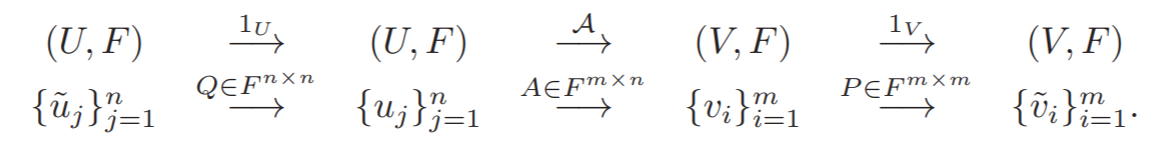
\includegraphics[width=\linewidth]{pictures/basis.png}
\end{Figure}


\textbf{Change of basis}: $ \mathcal{A}* = P \cdot A \cdot Q $

\section{3. Analysis}
\textbf{Norm}:1.$\forall v_1,v_2 \in V, \parallel v_1+v_2 \parallel \leq \parallel v_1 \parallel + \parallel v_2 \parallel$\\
2.$\forall v \in V, \forall a \in F, \parallel av \parallel =|a| \cdot \parallel v \parallel$\\
3.$\parallel v \parallel = 0 \Leftrightarrow v=0$\\
\textbf{Normed Linear Space}: $(V,F,\parallel \cdot \parallel)$\\
$\parallel x \parallel_1 = \sum_{i=1}^{n} |x_i|,$\\
$\parallel x \parallel_2 = \sqrt{\sum_{i=1}^{n} |x_i|^2},$\\
$\parallel x \parallel_p = (\sum_{i=1}^{n} |x_i|^p)^{\frac{1}{p}},$\\
$\parallel x \parallel_\infty = max |x_i|.$\\

\textbf{Ball}: Given $(V,F,\parallel \cdot \parallel)$, the \textbf{ball} of radius $r \in \mathbb{R}_+$ centered at $v \in V$ is $B(v,r) = \{ v' \in V | \parallel v - v' \parallel \leq r\}$.\\
$B(0,1) is$ \textbf{unit ball}.\\
\textbf{Bound}: $S \subseteq V$ is \textbf{bounded} if $S \subseteq B(0,r)$ for some r.\\
\textbf{Convergence}: Let (V, F, $\parallel \cdot \parallel$) be a normed space. A function v : N → V is called a sequence in V. The sequence converges to a point $\overline{v} \in V$ iff $\forall \epsilon > 0, \exists N \in \mathbb{N}, \forall m \geq N, \parallel v(m)-\overline{v} \parallel < \epsilon$\\

In this case, $\overline{v}$ is the \textbf{limit} of the sequence.\\
\textbf{Close}: iff all a set contains all its limit points.\\
\textbf{Open}: iff V\ K is closed.\\

\textbf{Compact}: Closed + Bounded.\\

\textbf{Continuous}: f is continuous at $u \in U$ iff
$\forall \epsilon > 0\ \exists \delta >0 s.t. \parallel u-u' \parallel_U < \delta \rightarrow \parallel f(u)-f(u') \parallel_U < \epsilon $.\\
$f$ is continuous on U iff it's continuous everywhere.\\
*All linear functions between finite dimensional spaces are always continuous.\\

\textbf{Equivalence}:Consider a L.S. (V, F) with two norms, $\parallel \cdot \parallel_a$ and $\parallel \cdot \parallel_b$.. Th two norms are equivalent iff\\
$\exists m_u \geq m_l \geq 0, \forall v \in V\ m_l\parallel v \parallel_a \leq \parallel v \parallel_b \leq \parallel v \parallel_a$.\\ 

\textbf{Weierstrass Theorem}: If $f: S \rightarrow \mathbb{R}$ is \underline{continuous} and set S is \underline{compact}, then $f$ attains a minimum on $S$.\\

\textbf{Cauchy Inequality}: $ (\sum_{i=1}^{n} a_i b_i)^{2} \leq (\sum_{i=1}^{n} a_i^2)(\sum_{i=1}^{n} b_i^2) $\\
Any two norms on a finite-dimensional space V are equivalent.\\

\textbf{Infinite-dimensional normed space}: \\
$\parallel f(t) \parallel_1 = \int_{t_0}^{t_1} \parallel f(t) \parallel_2 \,dt,$\\
$\parallel f(t) \parallel_2 = \sqrt{\int_{t_0}^{t_1} \parallel f(t) \parallel_2 ^2 \,dt},$\\
$\parallel f(t) \parallel_p = (\int_{t_0}^{t_1} \parallel f(t) \parallel_2 ^p \,dt)^{\frac{1}{p}},$\\
$\parallel f(t) \parallel_\infty = max \parallel f(t) \parallel_2.$\\
*Replacing $\parallel f(t) \parallel_2$ by another norm on $\mathbb{R}^n$ in the $\int_{t_0}^{t_1} \,dt$ and the $max$ are equivalent to the ones above.\\

\textbf{Cauchy Sequence}: $\{v_i\}_{i=0} ^\infty$ is a C.S. iff\\
$\forall \epsilon >0\ \exists N \in \mathbb{N}\ \forall m \geq N, \parallel v_m-n_N \parallel < \epsilon$.\\
*Every convergent Sequence is Cauchy.\\

\textbf{Complete}: The normed space $(V, F, \parallel \cdot \parallel)$ is complete (or \textbf{Banach}) iff every Cauchy sequence converges.\\
*Let $F = \mathbb{R}$ or $F = \mathbb{C}$ and if $(V,F)$ is finite-dimensional. Then $(V,F,\parallel \cdot \parallel)$ is a Banach Space for any norm $\parallel \cdot \parallel.$\\
*Many function spaces might not be Banach, but $(C([t_0,t_1], \mathbb{R}^n), \mathbb{R}, \parallel \cdot \parallel_\infty)$ is a Banach space.

\textbf{Induced Norm}: $\parallel f \parallel = $ \(\sup_{u \neq 0}\) $ \frac {\parallel f(u) \parallel_V}{\parallel u \parallel_U}$\\
*$\parallel \mathcal{A} \parallel = $ \(\sup_{\parallel u \parallel_U = 1}\) $ \parallel \mathcal{A}(u) \parallel_V$\\
$\parallel A \parallel_1 = max_{j = 1,...,n} \sum_{i=1}^{m} |a_{ij}| $ (max column sum)
$\parallel A \parallel_2 = max_{\lambda \in SPEC[A^T A]} \sqrt{\lambda}$ (max singular value)
$\parallel A \parallel_\infty = max_{i = 1,...,m} \sum_{j=1}^{n} |a_{ij}| $ (max row sum)\\

* $\mathcal{A}$ is continuous $\Leftrightarrow $ $\mathcal{A}$ is continuous at 0 $\Leftrightarrow$
  \(\sup_{\parallel u \parallel_U = 1}\) $ \parallel \mathcal{A}(u) \parallel_V < \infty$, the induced norm $\parallel \mathcal{A} \parallel$ is well defined.\\
Consider continuous linear functions $\mathcal{A}, \tilde{\mathcal{A}}: (V,F,\parallel \cdot \parallel_V) \rightarrow (W,F,\parallel \cdot \parallel_W),\ \mathcal{B}: (U,F,\parallel \cdot \parallel_U) \rightarrow (V,F,\parallel \cdot \parallel_V)$:\\
1. $\forall v \in V, \parallel \mathcal(A)(v) \parallel_W \leq \parallel \mathcal{A} \parallel \cdot \parallel v \parallel_V$.\\
2. $\forall a \in F, \parallel a \mathcal(A) \parallel = |a| \cdot \parallel \mathcal{A} \parallel$.\\
3. $\parallel \mathcal{A} + \tilde{\mathcal{A}} \parallel \leq \parallel \mathcal{A} \parallel + \parallel \tilde{\mathcal{A}} \parallel$.\\
4. $\parallel \mathcal{A} \parallel = 0 \Leftrightarrow \mathcal{A}(v)=0 for all v \in V$.\\
5. $\parallel \mathcal{A} \circ \mathcal{B} \leq \parallel \mathcal{A} \parallel \cdot \parallel \mathcal{B} \parallel$.\\

A function is \textbf{piecewise continuous} iff it's continuous at all $t \in \mathbb{R}$ except those in a set of discontinuity points $D \subseteq \mathbb{R}$ that satisfiy:\\
1. $\forall \tau \in D$ left and right limits of u exist, i.e. $lim_{t\rightarrow \tau^+} u(t)$ and $lim_{t\rightarrow \tau^-} u(t)$ exist and are finite. Moreover, $u(\tau) = lim_{t\rightarrow \tau^+} u(t)$.\\
2. $\forall t_0,t_1 \in \mathbb{R}$ with $t_0<t_1$, $D\cap [t_0, t_1]$ contains a finite number of points.\\

The function $p: \mathbb{R}^n \times \mathbb{R} \rightarrow \mathbb{R}^n$ is \textbf{globally Lipschitz} in x iff there exists a piecewise continuous function $k: \mathbb{R} \rightarrow \mathbb{R}_+$ s.t.\\
$\forall x,x' \in \mathbb{R}^n, \forall t\in\mathbb{R}\ \parallel p(x,t)-p(x',t) \parallel \leq k(t)\parallel x - x' \parallel$.\\

\textbf{Existence and uniqueness} Assume $p: \mathbb{R}^n \times \mathbb{R} \rightarrow \mathbb{R}^n$ is piecewise continuous w.r.t. its second argument (with discontinuity set $D \subseteq \mathbb{R}$) and globally Lipschitz w.r.t. its first argument. Then for all $(t_0,x_0) \in \mathbb{R} \times \mathbb{R}^n$ there exists a unique continuous function $\phi: \mathbb{R} \times \mathbb{R}^n$ s.t.:\\
1. $\phi(t_0) = x_0$.\\
2. $\forall t \in \mathbb{R} \backslash D, \frac{d}{dt} \phi(t) = p(\phi(t),t)  $.\\ 

*Let $\parallel \cdot \parallel$ be any norm on $\mathbb{R}^n$. Then for all $t_0,t_1 \in \mathbb{R},$\\
$\parallel \int_{t_0}^{t_1} f(t) dt \parallel \leq | \int_{t_0}^{t_1} \parallel f(t) \parallel dt |$\\
*1. $\forall m,k \in \mathbb{N}, (m+k)! \geq m!k!.$\\
*2. $\forall c \in \mathbb{R}, lim_{m \rightarrow \infty} \frac{c^m}{m!}=0.$\\
\textbf{Gronwall}: Consider $u(.),k(.): \mathbb{R} \rightarrow \mathbb{R}_+$ piecewice continuous, $c_1 \geq 0,$ and $t_0 \in \mathbb{R}$. If for all $t \in \mathbb{R}$, we have $u(t) \leq c_1 + |int_{t_0}^{t}k(\tau)u(\tau) d\tau|$. Then for all $t \in \mathbb{R}$, $u(t) \leq c_1exp|int_{t_0}^{t}k(\tau) d\tau|$.\\
\textbf{Autonomous Systems}: does not depends explicitly on time, $\dot{x}(t) = p(x(t))$.\\
*$s(t,t_0,x_0) = s(t-t_0,0,x_0)$




\newpage
\section{4. Time varying linear systems}
$\dot{x}(t) = f(x(t), u(t)) = A(t)x(t) + B(t)u(t)$ \qquad (1)\\
$y(t) = h(x(t), u(t)) = C(t)x(t) + D(t)u(t)$ \qquad (2)\\
where $x(t) \in \mathcal{R}^n$, $u(t) \in \mathcal{R}^m$, $x(t) \in \mathcal{R}^p$, \\
$A(\cdot):  \mathcal{R} \rightarrow \mathcal{R}^{n \times n}$, $B(\cdot):  \mathcal{R} \rightarrow \mathcal{R}^{n \times m}$, $C(\cdot):  \mathcal{R} \rightarrow \mathcal{R}^{p \times n}$, $D(\cdot):  \mathcal{R} \rightarrow \mathcal{R}^{p \times m}$ \\
\textbf{Linearization perturbation}\\
$x(t) = x^*(t) + e_x(t)$, $y(t) = x^*(t) + e_y(t)$\\
\textbf{Taylor extension of LVT}
$\dot{x}(t) = f(x^*(t)+e_x(t), u^*(t)+e_u(t))=f(x^*(t), u^*(t))+\frac{\partial{f}}{\partial{x}}(x^*(t), u^*(t))e_x(t)+\frac{\partial f}{\partial u}(x^*(t), u^*(t))e_u(t)$  + higher order terms\\
where 
$
\frac{\partial{f}}{\partial{x}}(x^*(t), u^*(t)) = \left[ \begin{array}{ccc} \frac{\partial{f_1}}{\partial{x_1}}(x^*(t), u^*(t)) & \cdots & \frac{\partial{f_1}}{\partial{x_n}}(x^*(t), u^*(t))\\
\vdots & \ddots & \vdots \\
\frac{\partial{f_n}}{\partial{x_1}}(x^*(t), u^*(t)) & \cdots & \frac{\partial{f_n}}{\partial{x_n}}(x^*(t), u^*(t))
\end{array} \right] = A(t)
$,\\
$
\frac{\partial{f}}{\partial{u}}(x^*(t), u^*(t)) = \left[ \begin{array}{ccc} \frac{\partial{f_1}}{\partial{u_1}}(x^*(t), u^*(t)) & \cdots & \frac{\partial{f_1}}{\partial{u_m}}(x^*(t), u^*(t))\\
\vdots & \ddots & \vdots \\
\frac{\partial{f_n}}{\partial{u_1}}(x^*(t), u^*(t)) & \cdots & \frac{\partial{f_n}}{\partial{u_m}}(x^*(t), u^*(t))
\end{array} \right] = B(t)
$\\
$\frac{d}{dt}(e_x(t))=A(t)e_x(t)+B(t)e_u(t)$\\
\textbf{Existence and structure of solutions}
\begin{tabular}{|c|c|c|c|}
\hline
 & $(X, \mathbb{R})$ & $(U, \mathbb{R})$ & $(Y, \mathbb{R})$\\
\hline
base & $ \{ e_i \}_{i=1}^n $ & $\{f_i\}_{i=1}^m $ & $\{g_i\}_{i=1}^p $\\
\hline
dim. & n & m & p\\
\hline
\end{tabular}\\
\textit{Assump 4.1}: $A(\cdot)$, $B(\cdot)$, $C(\cdot)$, $D(\cdot)$ are piecewise continuous.
\textit{Fact 4.1}: For all $u(\cdot): \mathbb{R} \rightarrow \mathbb{R}^m$ piecewise continuous and all $(t_0, x_0) \in \mathbb{R} \times \mathbb{R}_n$ there exists \textsc{unique} solution $x(\cdot):  \rightarrow \mathbb{R}^n$ and $y(\cdot):  \rightarrow \mathbb{R}^p$ for the system (1) and (2).\\
The unique solution of (1) and (2)\\
\textbf{State transition matrix}: $x(t) = s(t, t_0, x_0, u)$,\\
\textbf{Output response map}: $y(t) = \rho(t, t_0, x_0, u)$
% `\end` statements to match the `\begin`s.
\end{multicols*}

\end{document}